\documentclass[12pt]{article}
\usepackage[T1]{fontenc}
\usepackage[fleqn]{amsmath}
\usepackage{amssymb,amsfonts,amsthm,textcomp,mathrsfs}
\usepackage[subfigure]{tocloft}
\usepackage[hang]{subfigure}
\usepackage[title,titletoc]{appendix}
\usepackage{array}
\usepackage[pdftex]{graphicx}
\usepackage{grffile}
\usepackage{rotating}
\usepackage[usenames]{color}
\usepackage{tabularx,supertabular}
\usepackage{multirow}
\usepackage{hhline}
\usepackage{fancyhdr}
\usepackage{natbib}
\usepackage{vruler}
\usepackage{sectsty}
\usepackage{ctable}
\usepackage[utf8]{inputenc}
\usepackage{nomencl}
\usepackage{float}
\makenomenclature

\usepackage{hyperref}
\usepackage[
    open,
    openlevel=2,
    atend
]{bookmark}[2011/12/02]

\floatstyle{plaintop}
\restylefloat{table}

\allsectionsfont{\normalsize\bfseries}
\renewcommand{\cftsecfont}{\normalfont}
\renewcommand{\cftsecleader}{\cftdotfill{\cftdotsep}}
\renewcommand{\cftsecpagefont}{\normalfont}

\renewcommand\rmdefault{ptm}
\hypersetup{colorlinks=true, linkcolor=black, citecolor=black, filecolor=black, urlcolor=black, pdftitle=A Portable and Embedded SSVEP BCI System: emBCI, pdfauthor=Ozan Caglayan, pdfsubject=, pdfkeywords={eeg} {bci} {ssvep}, pdfcreator=, pdfproducer=}

\newcommand\textstyleJournalNames[1]{\foreignlanguage{english}{\textrm{\textmd{\textit{#1}}}}}

\setcounter{secnumdepth}{3}
\newcommand\mysection[1]{\vspace*{-0.35cm}\section{#1}\vspace*{6pt}\thispagestyle{empty}}
\newcommand\mysubsection[1]{\subsection{#1}}
\newcommand\mysubsubsection[1]{\subsubsection{#1}}

\newtheorem{thm}{Theorem}[section]
\newtheorem{cor}[thm]{Corollary}
\newtheorem{lem}[thm]{Lemma}
\newtheorem{defin}[thm]{Definition}

\makeatletter
\newcommand\arraybslash{\let\\\@arraycr}
\makeatother

\newcommand\liststyleLi{
\renewcommand\labelitemi{${\bullet}$}
\renewcommand\labelitemii{${\circ}$}
\renewcommand\labelitemiii{${\blacksquare}$}
\renewcommand\labelitemiv{${\bullet}$}
}

\setlength\paperwidth{21cm}
\setlength\paperheight{29.7cm}
\setlength\voffset{-1in} %printer
\setlength\hoffset{-1in} %printer
\setlength\topmargin{1.5cm}
\setlength\oddsidemargin{3.5cm}
\setlength\textheight{23.7cm}
\setlength\textwidth{15cm}
\setlength\marginparsep{0cm}
\setlength\marginparwidth{0cm}
\setlength\footskip{1.1cm} %printer
\setlength\headheight{0,6cm}
\setlength\headsep{1,4cm}

\makeatletter
\newcommand\ps@Standard{
  \renewcommand\@oddhead{}
  \renewcommand\@evenhead{}
  \renewcommand\@oddfoot{}
  \renewcommand\@evenfoot{}
  \renewcommand\thepage{\arabic{page}}
}
\makeatother

\pagestyle{fancy}
\renewcommand{\headrulewidth}{0pt}
\renewcommand{\footrulewidth}{0pt}
\fancyhead{}
\fancyfoot{}


\makeatletter
\newcommand\captionof[1]{\def\@captype{#1}\caption}
\makeatother

\newcounter{MathFormule}[section]
\renewcommand\theMathFormule{\thesection \arabic{MathFormule}}
\renewcommand{\baselinestretch}{1.5}
\setlength{\parskip}{\baselineskip}
\setlength{\parindent}{0mm}
\renewcommand\arraystretch{1.2}

%\newenvironment{mytableenv}
%{\setlength{\abovecaptionskip}{24pt}
%\setlength{\belowcaptionskip}{-18pt}
%\centering}
%{\setlength{\abovecaptionskip}{0pt}
%\setlength{\belowcaptionskip}{0pt}
%\par}

\newenvironment{myfigureenv}
{\setlength{\abovecaptionskip}{-6pt}
\setlength{\belowcaptionskip}{24pt}
\centering}
{\setlength{\abovecaptionskip}{0pt}
\setlength{\belowcaptionskip}{0pt}
\par}

\setlength\jot{6pt}
\renewcommand{\theequation}{\thesection \arabic{equation}}
\numberwithin{equation}{section}
\numberwithin{figure}{section}
\numberwithin{table}{section}

\hyphenpenalty=500

\newcommand\mathspaceadjust{
\vspace{6mm}
\topsep=0pt
\partopsep=0pt
\abovedisplayskip=0pt
\abovedisplayshortskip=0pt
\belowdisplayskip=0pt
\belowdisplayshortskip=0pt
}
\mathspaceadjust

\title{}

\begin{document}

%\clearpage
\setcounter{page}{1}
\pagenumbering{roman}
\cfoot{\roman{page}}
\thispagestyle{empty}
{
\vspace*{-14mm}
\centering\textbf{TITLE}\\\vspace*{1.5mm}
\centering\textbf{TITLE CONT.}\\\vspace*{1.5mm}
\centering{(TITLE IN TURKISH)}\\\vspace*{1.5mm}
\vspace*{15.5mm}
\centering{by}\\\vspace*{1.5mm}
\centering\textbf{AUTHOR NAME, M.S.}\\
\vspace*{30pt}
\centering\textbf{Thesis}\\\vspace*{1.5mm}
\centering{Submitted in Partial Fulfillment}\\\vspace*{1.5mm}
\centering{of the Requirements}\\\vspace*{1.5mm}
\centering{for the Degree of}\\
\vspace*{30pt}
\centering\textbf{DOCTOR OF PHILOSOPHY}\\\vspace*{1.5mm}
\centering{in}\\\vspace*{1.5mm}
\centering\textbf{INDUSTRIAL ENGINEERING}\\\vspace*{1.5mm}
\centering{in the}\\\vspace*{1.5mm}
\centering\textbf{INSTITUTE OF SCIENCE AND EGINEERING}\\\vspace*{1.5mm}
\centering{of}\\\vspace*{1.5mm}
\centering\textbf{GALATASARAY UNIVERSITY}\\
\vspace*{30pt}
\centering{Supervisor: Assoc. Prof. Dr. Name}\\\vspace*{1.5mm}
\vspace*{28.5mm}
\centering{Month Year}\\
}

\clearpage
\setcounter{page}{1}
\pagenumbering{roman}
\cfoot{\roman{page}}
\thispagestyle{empty}
{
\vspace*{-7.5mm}
\centering\textbf{A PORTABLE AND EMBEDDED SSVEP BCI SYSTEM: emBCI}\\\vspace*{1.5mm}
\centering{(TAŞINABİLİR VE GÖMÜLÜ BİR SSVEP BBA SİSTEMİ: emBCI)}\\\vspace*{1.5mm}
\vspace*{19mm}
\centering{by}\\\vspace*{1.5mm}
\centering\textbf{Ozan ÇAĞLAYAN, B.S.}\\
\vspace*{30pt}
\centering\textbf{Thesis}\\\vspace*{1.5mm}
\centering{Submitted in Partial Fulfillment}\\\vspace*{1.5mm}
\centering{of the Requirements}\\\vspace*{1.5mm}
\centering{for the Degree of}\\
\vspace*{30pt}
\centering\textbf{MASTER OF SCIENCE}\\\vspace*{1.5mm}
\centering{in}\\\vspace*{1.5mm}
\centering\textbf{COMPUTER ENGINEERING}\\\vspace*{1.5mm}
\centering{in the}\\\vspace*{1.5mm}
\centering\textbf{INSTITUTE OF SCIENCE AND ENGINEERING}\\\vspace*{1.5mm}
\centering{of}\\\vspace*{1.5mm}
\centering\textbf{GALATASARAY UNIVERSITY}\\
\vspace*{60pt}
\vspace*{16.5mm} %printer
\centering{January 2014}\\
}

\clearpage
\setcounter{page}{1}
\pagenumbering{roman}
\cfoot{\roman{page}}
\thispagestyle{empty}
{
\vspace*{-7.5mm}
\centering\textbf{A Portable and Embedded SSVEP BCI Application: emBCI}\\\vspace*{1.5mm}
%\centering\textbf{TITLE CONT.}\\\vspace*{1.5mm}
\centering{(Taşınabilir ve Gömülü bir SSVEP BBA Uygulaması: emBCI)}\\\vspace*{1.5mm}
\vspace*{13mm}
\centering{by}\\\vspace*{1.5mm}
\centering\textbf{Ozan ÇAĞLAYAN, B.S.}\\
\vspace*{30pt}
\centering\textbf{Thesis}\\\vspace*{1.5mm}
\centering{Submitted in Partial Fulfillment}\\\vspace*{1.5mm}
\centering{of the Requirements}\\\vspace*{1.5mm}
\centering{for the Degree of}\\
\vspace*{30pt}
\centering\textbf{MASTER OF SCIENCE}\\
\vspace*{10pt}
\begin{alignat*}{2}
 & \quad\quad\quad\quad\quad\text{Date of Submission \quad } && \text{: Month Day, Year} \\
 & \quad\quad\quad\quad\quad\text{Date of Defense Examination \quad } && \text{: Month Day, Year}
\end{alignat*}
\vspace*{10pt}
\begin{alignat*}{2}
 & \text{Supervisor} && \text{: Assist. Prof. Dr. R. Burak ARSLAN} \\
 & \text{Committee Members \quad } && \text{: Assoc. Prof. Dr. Name} \\
 & \text{} && \text{\; Prof. Dr. Name (Unv.)} \\
 & \text{} && \text{\; Assist. Prof. Dr. Name} \\
 & \text{} && \text{\; Assoc. Prof. Dr. Name (Unv.)}
\end{alignat*}
}

%%%%%%%%%%%%%%%%%%%%%%
%% ACKNOWLEDGEMENTS %%
%%%%%%%%%%%%%%%%%%%%%%
\clearpage
\vspace*{-0.35cm}
\section*{Acknowledgements}
\addcontentsline{toc}{section}{Acknowledgements}
\vspace*{6pt}
\par{
Back in 2007, I remember how I was fascinated when I had heard about Brain-Computer interfaces.
}
\par{
Last but not least, I would like to thank my family and my friends for supporting me throughout my life.
}
\par{
Finally, I would like to dedicate this thesis to Ethem Sarısülük, Mehmet Ayvalıtaş, Abdullah Cömert, Medeni Yıldırım, Ali İsmail Korkmaz,
Ahmet Atakan and Hasan Ferit Gedik who passed away during Gezi Protests.\\
\emph{"Our hearts shall wither if we ever forget."}
}

\vspace*{2cm}
\begin{flushright}
February 2014, Istanbul \\
Ozan Çağlayan
\end{flushright}
\clearpage

%%%%%%%%%%%%%%%%%%%%%%%
%% TABLE OF CONTENTS %%
%%%%%%%%%%%%%%%%%%%%%%%
\setcounter{tocdepth}{5}
\renewcommand\contentsname{\normalsize\bfseries Table of Contents}
\phantomsection
\thispagestyle{empty}
\vspace*{0.15cm}
\addcontentsline{toc}{section}{Table of Contents}
\tableofcontents
\clearpage

%%%%%%%%%%%%%%%%%%%%%
%% LIST OF SYMBOLS %%
%%%%%%%%%%%%%%%%%%%%%
\renewcommand\nomname{\normalsize\bfseries List of Abbreviations}
\phantomsection
\thispagestyle{empty}
\vspace*{0.15cm}
\addcontentsline{toc}{section}{List of Abbreviations}
\printnomenclature
\clearpage

%%%%%%%%%%%%%%%%%%%%%
%% LIST OF FIGURES %%
%%%%%%%%%%%%%%%%%%%%%
\renewcommand\listfigurename{\normalsize\bfseries List of Figures}
\phantomsection
\thispagestyle{empty}
\vspace*{0.15cm}
\addcontentsline{toc}{section}{List of Figures}
\listoffigures
\clearpage

%%%%%%%%%%%%%%%%%%%%
%% LIST OF TABLES %%
%%%%%%%%%%%%%%%%%%%%
\renewcommand\listtablename{\normalsize\bfseries List of Tables}
\phantomsection
\thispagestyle{empty}
\vspace*{0.15cm}
\addcontentsline{toc}{section}{List of Tables}
\listoftables
\clearpage

%%%%%%%%%%%%%%
%% ABSTRACT %%
%%%%%%%%%%%%%%
\vspace*{-0.35cm}
\thispagestyle{empty}
\section*{Abstract}
\addcontentsline{toc}{section}{Abstract}
\vspace*{6pt}

\par{
Abstract abstract abstract.
}
\clearpage

%%%%%%%%%%%%
%% RESUME %%
%%%%%%%%%%%%
\vspace*{-0.35cm}
\thispagestyle{empty}
\section*{R\'{e}sum\'{e}}
\addcontentsline{toc}{section}{R\'{e}sum\'{e}}
\vspace*{6pt}

\par{
Resume resume resume.
}
\clearpage

%%%%%%%%%%
%% OZET %%
%%%%%%%%%%
\vspace*{-0.35cm}
\thispagestyle{empty}
\section*{\"{O}zet}
\addcontentsline{toc}{section}{\"{O}zet}
\vspace*{6pt}

\par{
Ozet ozet ozet.
}
\clearpage

%%%%%%%%%%%%%%%%%%
%% INTRODUCTION %%
%%%%%%%%%%%%%%%%%%
\mysection{INTRODUCTION}
\thispagestyle{fancy}
\pagenumbering{arabic}
\chead{\arabic{page}}
\cfoot{}
\par{
The objective of a brain-computer interface is to provide an alternative way of interaction between the brain and the environment
without the involvement of muscular pathways. Besides being a revolutionary human computer interface for gaming and entertainment,
BCIs constitute the only way of interaction/communication with the outer world for people who cannot voluntarily control/move their muscles.
}
\par {
Electroencephalography is a non-invasive method for measuring the electrical activity generated within the brain structures, through the scalp.
Although an electrode placed on the scalp measures a linear mixture of various electrical sources underlying the electrode site,
we can deduce some informations from those measurements using various signal processing and pattern recognition techniques.
}
\clearpage

%%%%%%%%%%%%%%%%%%
%% SECTION: BCI %%
%%%%%%%%%%%%%%%%%%
\mysection{BRAIN COMPUTER INTERFACES}\label{seq:bci}

\par{
    \nomenclature{LIS}{Locked-in Syndrome}
    \nomenclature{ALS}{Amyotrophic Lateral Sclerosis}
    The locked-in syndrome (LIS) is a medical condition in which patients are awake and conscious but
    cannot move or communicate verbally because of complete paralysis of nearly all voluntary muscles.
    LIS is mostly caused by traumatic brain injuries, brain strokes, hemorrhages, head trauma, demyelinating diseases
    or infectious conditions. Amyotrophic Lateral Sclerosis (ALS) (Also known as Lou Gehrig's disease,
    named after a popular baseball player who was diagnosed with ALS in 1939) is a neurodegenerative disease
    which is one of the major causes of LIS. ALS basically attacks motor neurons that control voluntary muscles in the body.
    When those motor neurons stops functioning, the muscles lose strength and progressively die (Atrophy).
    A cure for ALS is currently not available and the cause of the disease is still unknown.
}

\par {
    According to ALS Association, nearly 5600 people in the United States are
    diagnosed with ALS each year and the incidence of the disease is 2 per 100.000
    people\footnote{\url{http://www.alsa.org/about-als/facts-you-should-know.html}}. Although
    there doesn't seem to be an incidence study related to ALS in Turkey, it is estimated that
    6000-8000 people have the disease.\footnote{\url{http://www.als.org.tr/haber_detay.asp?haberID=77}}.
}

\par{
    \nomenclature{BCI}{Brain-Computer Interface}
    \nomenclature{HCI}{Human-Computer Interaction}
    \nomenclature{BMI}{Brain-Machine Interface}
    \nomenclature{DBI}{Direct Brain Interface}
    When consciousness and cortical functions are preserved, it may actually be
    possible to use healthy brain activity in order to build a novel way of interaction
    between the subject's brain and the environment using special brain signal
    acquisition techniques and computers. These composite systems are called
    Brain-Computer Interfaces (BCI), Brain-Machine Interfaces (BMI) or Direct Brain Interfaces (DBI).
    BCIs in general have the potential to improve the life quality of disabled people and may actually
    be the only way of interaction for completely locked-in people.
}

\mysubsection{Definition of a BCI}\label{seq:bci_definition}
\par{
    According to \citet{wolpaw_braincomputer_2002}, a BCI is a communication system
    in which messages or commands sent to the external world do not pass through the
    brain's normal neuromuscular output pathways; thus BCIs provide an alternative
    way for people to act on the world.
}
\par{
    Three mandatory elements for a BCI system has further been enumerated by \citet{graimann_braincomputer_2010}:
    \begin{enumerate}
        \item A BCI must directly record brain activity,
        \item A BCI must provide \emph{realtime} feedback to the user,
        \item A BCI must be based on intentional control.
    \end{enumerate}
    The \emph{intentional control} constraint mentioned above, leaves the devices
    that detect changes in brain activity occurring without any intent like
    workload, arousal or sleep, out of the definition for BCIs.
}
\par{
    A more application-focused definition from the perspective of
    Human-Computer Interaction (HCI) proposed by \citet{zander_enhancing_2010}
    is as follows:
    \quotation{\emph{"A BCI is a system to provide computer applications with access to real-time
    information about cognitive state, on the basis of measured brain activity."}}
}
\par{
    \citet{zander_enhancing_2008} also categorized BCIs into three types:
    \begin{itemize}
        \item \emph{Active BCI} A BCI deriving its outputs from consciously controlled brain activity.
        \item \emph{Reactive BCI} A BCI deriving its outputs from brain activity arising in response to external stimuli.
        \item \emph{Passive BCI} A BCI deriving its outputs from arbitrary brain activity without the purpose of voluntary control.
    \end{itemize}
    According to this categorization, passive BCIs embrace the systems
    based on arbitrary activity detection which were not previously counted as BCIs by \citet{graimann_braincomputer_2010}.
}

\mysubsection{Neural Principles}\label{seq:neural_principles}
\mysubsubsection{Central Nervous System}\label{seq:neural_principles_cns}
\par{
%linear mixture of sources, belki biraz source localization,
    \nomenclature{CNS}{Central Nervous System}
    \nomenclature{PNS}{Peripheral Nervous System}
    \nomenclature{M1}{Primary Motor Cortex}
    \nomenclature{V1}{Primary Visual Cortex}
    The central nervous system (CNS) is the part of the nervous system which
    integrates sensory information it receives from the body and responds to it accordingly.
    Together with the peripheral nervous system (PNS) which connects CNS to the
    limbs and organs, it plays an important role in determining the behavior. The two
    structures that make up the CNS are the brain and the spinal cord which is the
    information pathway containing nervous tissue that extends from the brain.
}
\par{
    The human brain is divided into two (left and right) cerebral hemispheres
    covered with \emph{cortex} which is also known as the \emph{gray matter},
    the type of CNS tissue made of neurons. The hemispheres are connected
    through a central structure called \emph{corpus callosum} which is a bundle
    of neural fibers that enables the communication between hemispheres.
}

\par{
    Each cerebral hemisphere is further divided
    into frontal, parietal, occipital and temporal lobes (Figure ~\ref{fig:brain_parts})
    which have specialized functions (Table ~\ref{table:brain_functions}) driving our cognitive abilities.
    It should be noted that each hemisphere is primarily involved in sensory and motor processes on
    the opposite side of the body and the "apparently" similar cerebral hemispheres are
    neither functionally equivalent nor exactly symmetrical \citep{kandel_principles_2013}.

\begin{table}[H]
    \footnotesize
    \centering
    \caption{Functional description of cerebral lobes.}
    \begin{tabular}{l l}
        \hline
        Frontal Lobe & Executive functions, movement control \emph{(Primary motor cortex (M1))}\\ \hline
        Parietal Lobe & Multimodal sensory information integration \\ \hline
        Occipital Lobe & Visual processing center containing the \emph{visual cortex (V1)} \\ \hline
        Temporal Lobe & Hearing and auditory signal processing, memory, emotion\\ \hline
    \end{tabular}
    \label{table:brain_functions}
\end{table}

\begin{figure}[ht]
    \centering
    \includegraphics[scale=0.5]{images/Cerebrum_lobes}
    \caption[Functional regions of the cerebral cortex.]{Functional regions of the cerebral cortex. (Adapted from \href{http://en.wikipedia.org/wiki/File:Cerebrum_lobes.svg}{Wikipedia})}
    \label{fig:brain_parts}
\end{figure}
}

\mysubsubsection{Neurons}\label{seq:neural_principles_neurons}

\par{
    Neurons or nerve cells are the core components of the brain. There are
    approximately 10\textsuperscript{11} neurons in the human brain \citep{kandel_principles_2013}
    forming complex interconnected networks to produce human behavior.

\begin{figure}[ht]
    \centering
    \includegraphics[scale=0.9]{images/neuron}
    \caption[The structure of a neuron.]{The structure of a neuron. (Adapted from \href{http://commons.wikimedia.org/wiki/File:Neuron.svg}{Wikipedia})}
    \label{fig:neuron}
\end{figure}
}

\par{
    A typical neuron is composed of four regions: The cell body or soma, dendrites, axon
    and presynaptic terminals (Figure ~\ref{fig:neuron}).
}
\par{
    The cell body, surrounded by a membrane made of lipid layers, is the center
    of the neuron containing the nucleus which is responsible for protein synthesis.
    A number of short branches called \emph{dendrites} extend from the cell body. The function
    of dendrites is to receive incoming signals sent by other neurons. In contrast to having
    multiple dendrites for input, neurons have a single tubular output extension called \emph{axon}.
    This single axon branches out into extremities known as \emph{presynaptic terminals} which
    transmit the electrical signal to the (postsynaptic) dendrites of other neurons (postsynaptic cells)
    using special chemicals called \emph{neurotransmitters}. The zone where these presynaptic terminals
    and postsynaptic dendrites communicate with the help of neurotransmitters is called the \emph{synapse}.
    An axon has the ability to carry signals over distances
    between \emph{0.1mm} and \emph{2m} \citep{kandel_principles_2013}.
}

\par{
    \begin{figure}[ht]
        \centering
        \includegraphics[scale=0.4]{images/ap}
        \caption[Action potential.]{Action potential. \citep{sanei_eeg_2008}}
        \label{fig:action_pot}
    \end{figure}

}

\par{
    \nomenclature{EEG}{Electroencephalography}
    \nomenclature{MEG}{Magnetoencephalography}
    When neurons are activated, synaptic currents are produced within the dendrites.
    The magnetic and electric fields generated by these currents can be
    measured by Magnetoencephalography (MEG) and Electroencephalography (EEG) \citep{sanei_eeg_2008}.
}

%\mysubsection{History}\label{seq:bci_history}

%\begin{figure}[ht]
%    \centering
%    
\includegraphics[scale=1.0]{images/motor_areas}
%    \caption{Hand and foot areas in brain.}
%    \label{fig:motor_functions}
%\end{figure}

% EEG, ECoG, Intracortical, MEG, fMRI, NIRS
\mysubsection{Signal Acquisition Methods}\label{seq:bci_methods}
\par{
    \begin{figure}[ht]
        \centering
        \includegraphics[scale=0.5]{images/eeg_vs_ecog}
        \caption[Comparison of EEG, ECoG and Intracranial Recordings.]{Comparison of EEG, ECoG and Intracranial Recordings. (Drawing courtesy of B. Blankertz)}
        \label{fig:methods_eeg_ecog}
    \end{figure}
}
\mysubsubsection{EEG}\label{seq:bci_methods_eeg}
\mysubsubsection{ECoG}\label{seq:bci_methods_ecog}
\mysubsubsection{Intracortical Recordings}\label{seq:bci_methods_intracortical}
\mysubsubsection{fMRI}\label{seq:bci_methods_fmri}
\mysubsubsection{fNIRS}\label{seq:bci_methods_fnirs}

\mysubsection{Principles of EEG}\label{seq:eeg_principles}

\mysubsubsection{Electrode Placement}\label{seq:eeg_placement}
\par{
Human EEG is recorded using an internationally recognized electrode naming and placement
standard called 10-20 system \citep{jasper_ten_1958} (Figure ~\ref{fig:eeg_1020}).
This standard is based on the relationship between electrode locations and the underlying
area of the brain. A combination of a letter and a number is further used to identify each electrode location.
}

\begin{figure}[ht]
    \centering
    \includegraphics[scale=0.65]{images/10_20_bembook1}
    \caption[International 10-20 system.]{International 10-20 system. \citep{malmivuo_bioelectromagnetism:_1995}}
    \label{fig:eeg_1020}
\end{figure}

\par{
    The letters \emph{F, Fp, T, C, P} and \emph{O} respectively denotes \textbf{F}rontal, \textbf{F}ronto\textbf{P}olar
    (or \textbf{F}rontal \textbf{P}olar), \textbf{T}emporal, \textbf{C}entral, \textbf{P}arietal and
    \textbf{O}ccipital lobes. (Note that the \emph{C} letter is only meaningful as a notation to define the central line
    as the brain does not have an area called central lobe.) An A is used to refer to earlobes.
    Electrodes over the left hemisphere are suffixed with odd numbers and those over the right hemisphere
    are suffixed with even numbers. A \emph{"z"} instead of a number refers to an electrode placed on the midline, which
    is named the \emph{vertex}.
}

\par{
    Two anatomical landmarks are used to define the longitudinal axis over the scalp: First, the \emph{Nasion (Ns or Nz)}, which is the
    depressed area between the eyes where the bridge of the nose joins the forehead; second, the \emph{Inion (In or Iz)}, which is
    indicated by a bump at the lower rear part of the skull. From these landmarks, Ns-In perimeters are divided into 10\% and 20\% intervals
    and electrode locations are fixed at those division points. Three other electrodes are placed on each hemisphere
    (F3,C3,P3 and F4,C4,P4) equidistantly from the already placed adjacent electrodes. The percentage of division intervals
    clearly reveals why the system is named after the term 10-20.
}

\par{
    Another widely used electrode placement schema is the full 10-10 combinatorial
    system \citeyearpar{guideline_1994} which is a sophisticated 10-20
    variant with more and more electrodes placed in between 10-20 locations
    (Figure ~\ref{fig:eeg_1020_comb}\footnote{Image courtesy of Marius 't Hart (\url{http://www.mariusthart.net/?e=200})}).
    New letters are introduced to define intermediate electrode sites: \emph{AF} is between Fp and F, \emph{FC} is between F and C,
    \emph{FT} is between F and T, \emph{CP} is between C and P, \emph{TP} is between T and P, and finally \emph{PO} is between P and O.
    The colored locations are actually T3, T4, T5 and T6 electrodes in 10-20 system but
    they are renamed to T7, T8, P7 and P8 in this modified schema.
}

\par{
    A new 10-5 extension with 345 electrodes was also proposed by \citet{oostenveld_five_2001} for high resolution EEG studies.
}

\begin{figure}[ht]
    \centering
    \includegraphics[scale=0.6]{images/10_20_extended}
    \caption{10-10 combinatorial system.}
    \label{fig:eeg_1020_comb}
\end{figure}

\mysubsubsection{Montage and Recording}\label{seq:eeg_recording}
\par{
bipolar-unipolar recordings, referencing, 
electrode types (aktif, pasif, jel, dry, resim)
}

%%%%%%%%%%%%%
%% SECTION %%
%%%%%%%%%%%%%
\clearpage
\vspace*{-0.35cm}
\mysection{HARDWARE}\label{seq:hardware}

\mysubsection{Why Embedded Computer?}\label{seq:embeddedcomputer}

\par{
Single computer BCIs generally require decent computers as they can make use of heavy signal processing 
and machine learning algorithms while probably presenting visual stimuli in a precise timing.
}

\par{
Today, the embedded computers found on smartphones are much powerful compared to the desktop PCs
used in the BCI systems designed years ago. The main concern of this study is to assess whether small,
(possibly) battery-powered and cheap embedded computers can be used to replace big, power hungry and
expensive computers in a simple, online BCI system.
}

\mysubsubsection{Advantages}\label{seq:embeddedcomputer_advantages}

\par{
Majority of embedded computers runs Linux which does not require a graphical desktop environment
to be available. This allows to reduce memory and CPU usage on these systems as the most resource
hungry component of a modern operating systems is the Graphical User Interface (GUI).
}

\par{
Using Linux also helps to prepare a custom OS designed to run the BCI loop efficiently.
This is achieved by removing/disabling system services and applications which won't be required at all by BCIs.
}

\par{
All of these optimizations reduce the overall power consumption of the embedded BCI which brings
the possibility to use a battery-pack as power supply. This final achievement is key to ultimate
portability of BCI systems.
}

\mysubsection{BeagleBone Black}\label{seq:embeddedcomputer_bbb}

\par{
    \nomenclature{BBB}{BeagleBone Black}
BeagleBone Black (BBB) (Figure ~\ref{fig:bbb}) is a 45\$ single board computer released in 2013. It has 1GHz TI AM3359 Sitara ARM Cortex-A8 microprocessor,
512MB DDR3 memory, 3D accelerated PowerVR SGX530 graphical processing unit (GPU) with HDMI output, onboard 2GB embedded MMC (eMMC)
flash storage pre-loaded with Ångström Linux distribution. Along with a single USB 2.0 host port and 10/100 RJ45 Ethernet port for
general purpose connectivity, the board also provides a wide variety of low-level expansion interfaces:
4xUART, 8xPWM, 2xSPI, 1xADC and 2xI\textsuperscript{2}C.
}

\begin{figure}[ht]
    \centering
    \includegraphics[width=0.4\textwidth]{images/bbb}
    \caption{BeagleBone Black Single-board Computer.}
    \label{fig:bbb}
\end{figure}

\mysubsubsection{Programmable Realtime Unit}\label{seq:embeddedcomputer_bbb_pru}
\par{
    \nomenclature{PRU}{Programmable Realtime Unit}
    \nomenclature{OS}{Operating System}
    Although the Cortex-A8 processor is powerful, real-time control of high-speed external hardware
    and high precision tasks can be affected by operating system (OS) latencies. BBB improves the
    situation by providing two programmable realtime units (PRU) optimized to perform embedded tasks
    with hard realtime constraints. The PRUs have:
    \begin{itemize}
        \item Two 32-bit RISC cores running at 200MHz (Each instruction completes in 5ns)
        \item 8KB data memory and 8KB instruction memory
        \item 12KB shared memory
        \item A small instruction set
    \end{itemize}
    It is sometimes possible to encounter delays in OS scheduling while EEG
    acquisition and SSVEP stimulation are both running simultaneously. This can negatively
    impact the precision of flickering intervals causing the BCI to perform badly.
    Offloading SSVEP stimulation to the PRU resolves this problem as PRU is a distinct
    microcontroller unit which is completely decoupled from the main CPU of the device.
}
\par{
    By now, the PRU can only be programmed using assembly language. A helper library
    for C and Python is available to launch and terminate custom programs written for the PRU.
    It is also possible to share data between the PRU and the CPU using shared memory.
}

\mysubsubsection{Initial Setup and Customization}\label{seq:embeddedcomputer_initialsetup}
\par{
We first installed Ubuntu (into the onboard eMMC storage) as it is a widely adopted Linux distribution with a rich software repository. A rich software repository is important for avoiding 
manual compilation/installation of several tools and libraries, which in turn decreases time needed to start experimenting with the BCI system.
}

\par{
The list of tools and libraries that we'll be frequently using throughout this work are: {\em Git, python-emotiv, SciPy, NumPy, pycrypto, pyusb, python GPIO library for BBB.}
}

\par{
Several unused system services like BLAH, BLAH, BLAH are completely disabled so that they don't waste available system resources.
}

\mysubsubsection{Stimuli Generation on BBB}\label{seq:embeddedcomputer_stimuligen}
\par{
}
\par{
    In order to preserve the portability of the system, we decided to use BBB's
    Input/Output capabilities for LED SSVEP stimulation (Figure ~\ref{fig:bbb_led_schema}).
    BBB has several General-Purpose Input/Output (GPIO) pins that can be used to communicate with external
    devices and circuits. These pins can be raised HIGH (+3.3v) or LOW (0v)
    using Adafruit BBIO library\footnote{\url{https://github.com/adafruit/adafruit-beaglebone-io-python}} for Python.
}

\begin{figure}[ht]
    \centering
    \includegraphics[width=0.7\textwidth]{images/led_circuit}
    \caption{SSVEP LED stimulator schematic.}
    \label{fig:bbb_led_schema}
\end{figure}

\mysubsection{Emotiv EEG}\label{seq:emotiveeg}

\par{
    Emotiv EEG (Figure ~\ref{fig:emotiv_eeg_headset}) is a battery-powered wireless consumer headset which can
    acquire 14 channels (Figure ~\ref{fig:emotiv_eeg_1020}) of EEG signal. The headset internally applies a
    notch filter (At line frequency 50/60Hz) and a 5\textsuperscript{th} order band-pass filter (0.2-45Hz)
    to the signal. Although the internal sampling rate of the headset is 2048Hz, the device
    downsamples the signal to 128Hz before sending them to the computer. Full technical specifications found in the
    manufacturer's website\footnote{\url{http://www.emotiv.com/eeg/download_specs.php}} are summarized in Table ~\ref{table:emotiv_eeg_specs}.
}

\begin{figure}[ht]
    \centering
    \includegraphics[scale=0.6]{images/10_20_emotiv}
    \caption{Emotiv EEG Electrode Locations.}
    \label{fig:emotiv_eeg_1020}
\end{figure}

\begin{figure}[ht]
    \centering
    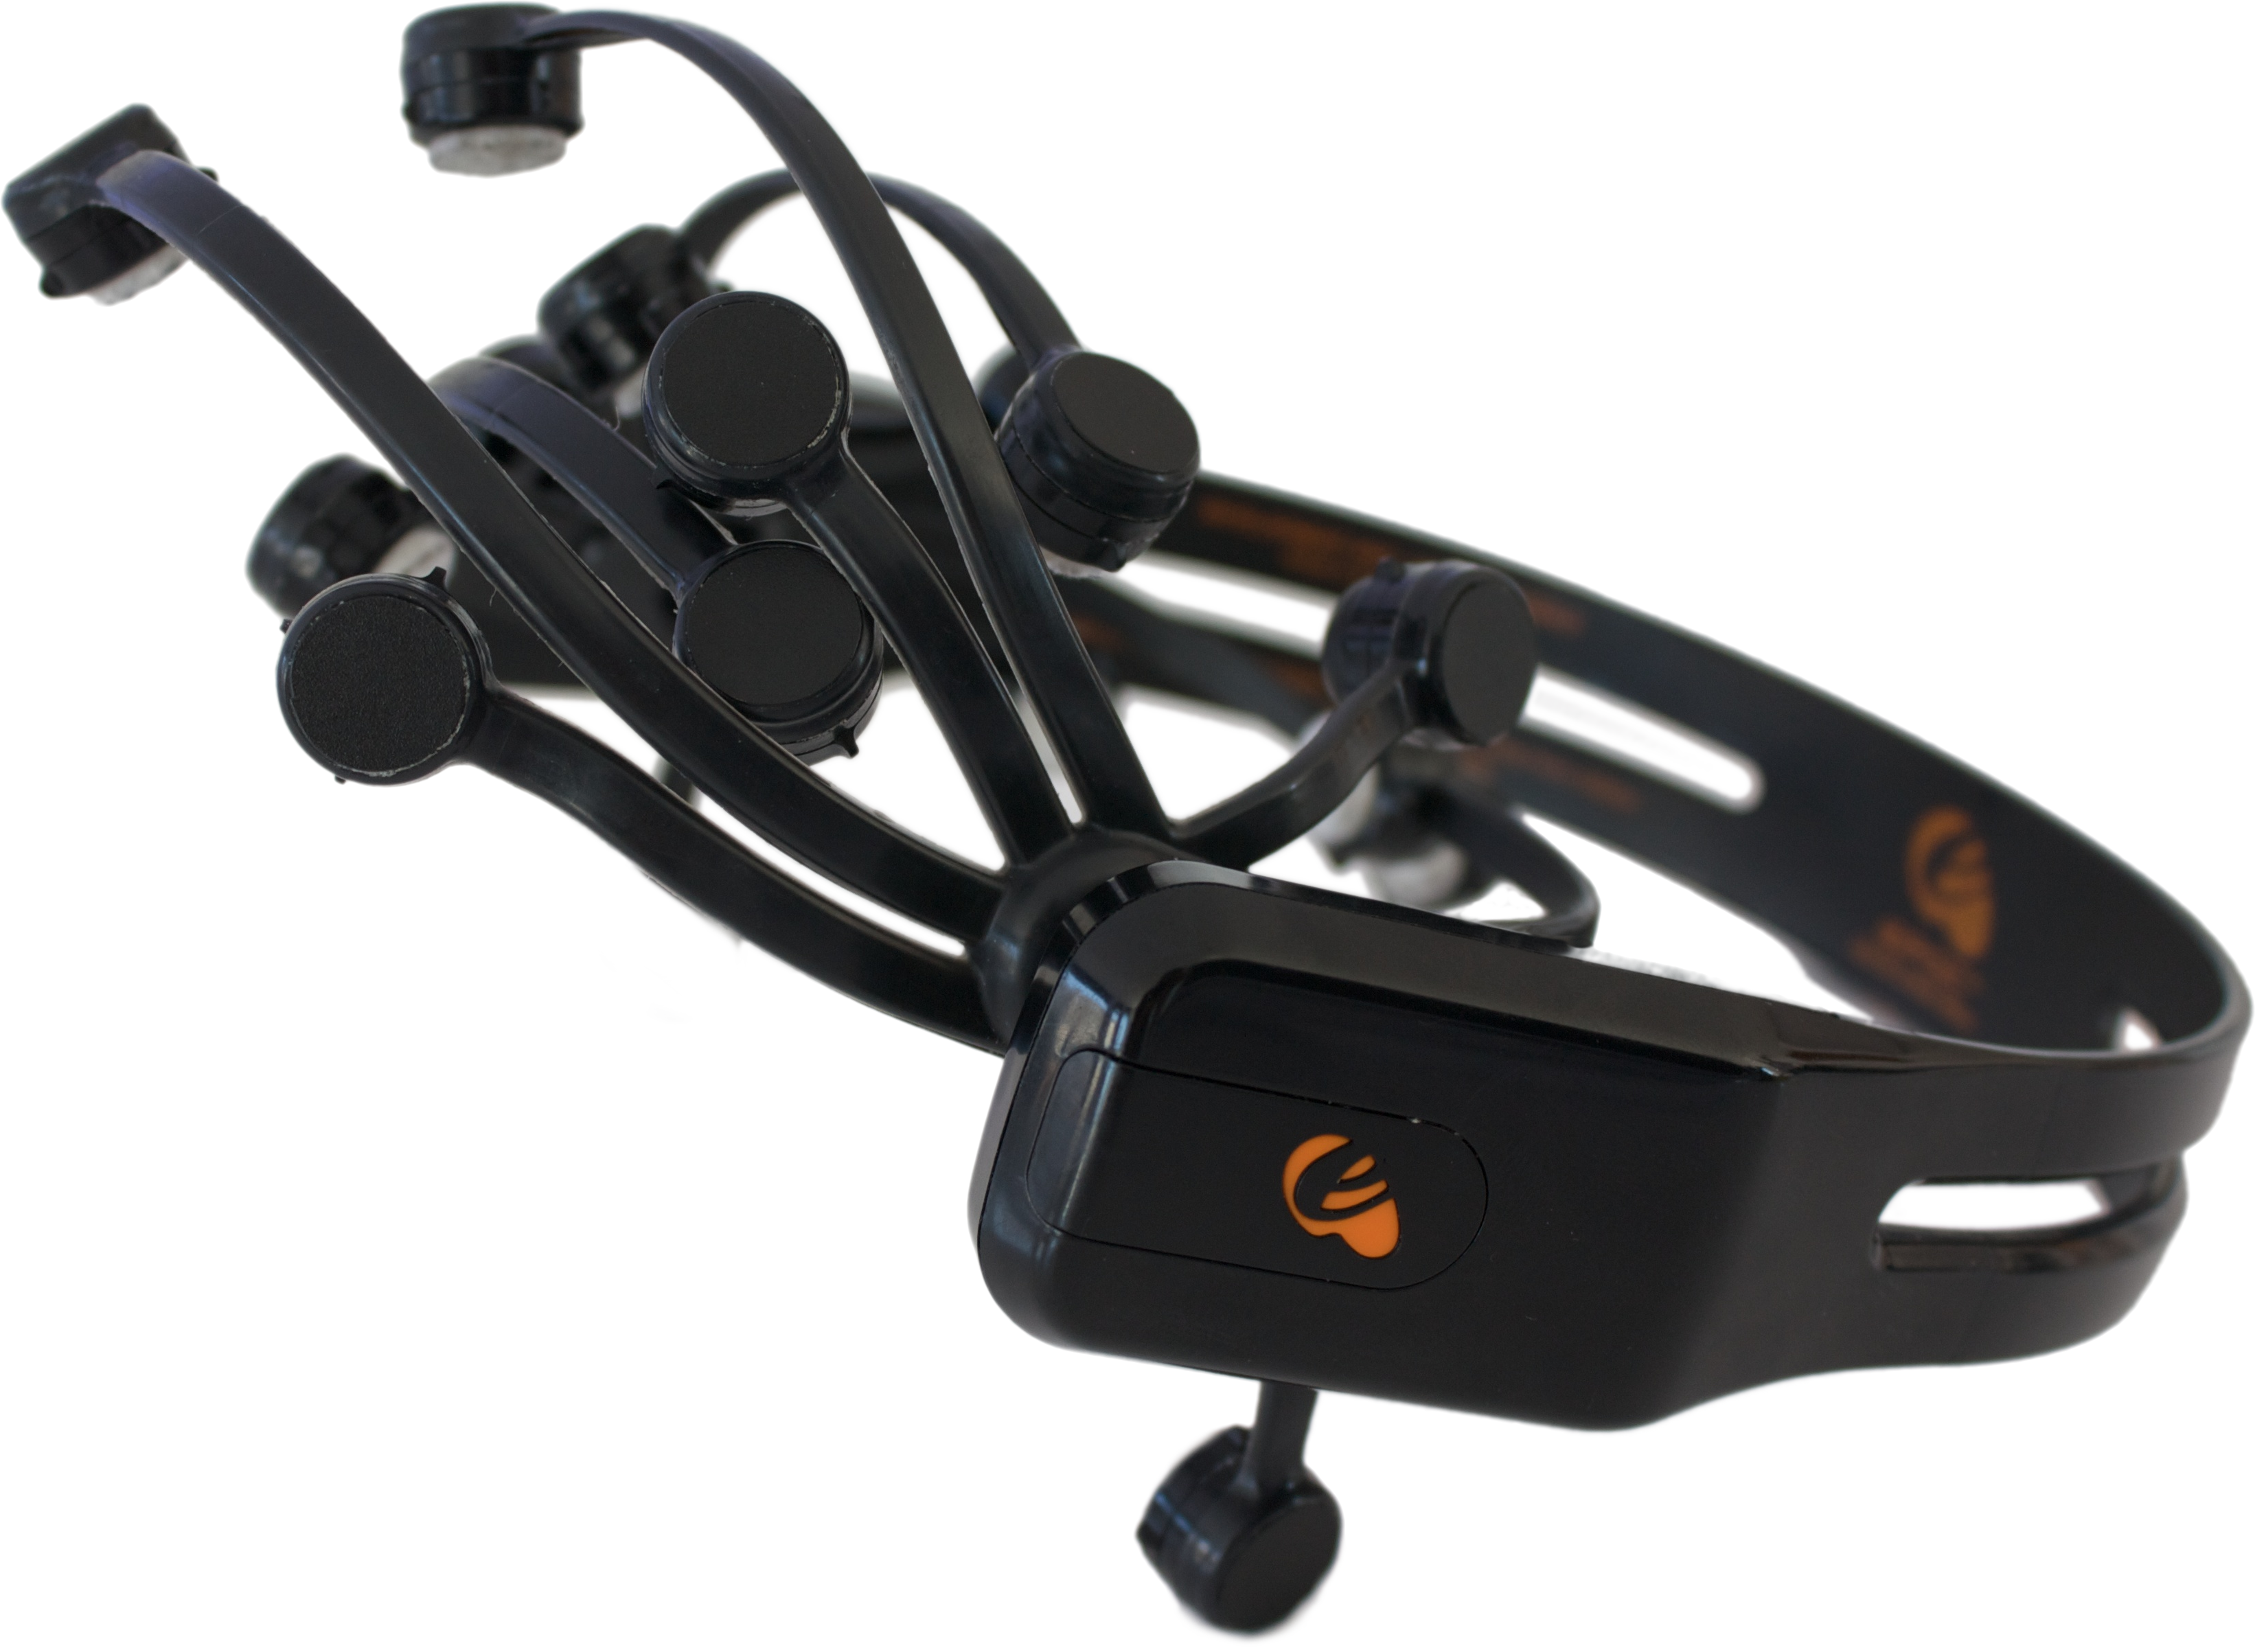
\includegraphics[width=0.5\textwidth]{images/emotiv}
    \caption{Emotiv EEG Headset.}
    \label{fig:emotiv_eeg_headset}
\end{figure}

\begin{table}
    \footnotesize
    \centering
    \caption{Technical specifications of Emotiv EEG.}
    \begin{tabular}{ll}
        \hline
        Number of channels & 14 (+ CMS/DRL references, P3/P4 locations) \\ \hline
        Channel names & AF3, F7, F3, FC5, T7, P7, O1, O2, P8, T8, FC6, F4, F8, AF4 \\ \hline
        Sampling method & Sequential sampling, single ADC \\ \hline
        Sampling rate & 128 SPS (2048 Hz Internal) \\ \hline
        Resolution & 14 bits 1 LSB = 0.51uV \\ \hline
        Bandwidth & 0.2-45Hz, digital notch filters at 50Hz and 60Hz \\ \hline
        Filtering & Built-in digital 5th order Sinc filter \\ \hline
        Dynamic range (input referred) & 8400uV (pp) \\ \hline
        Coupling mode & AC coupled \\ \hline
        Connectivity & Proprietary wireless, 2.4GHz band \\ \hline
        Battery life & 12 hours (typical) \\ \hline
        Impedance measurement & Real-time contact quality using patented system \\ \hline
    \end{tabular}
    \label{table:emotiv_eeg_specs}
\end{table}

\mysubsubsection{Official Software Development Kit (SDK)}\label{seq:emotiveeg_sdk}

\par{
Emotiv provides an SDK for Windows, Mac OS X and Linux operating systems but the provided SDK is
closed-source and only available for x86 CPU architecture. This means that it is not possible
to use the SDK on ARM embedded computers like Raspberry Pi or Beaglebone Black.
Currently, the only way of using the Emotiv headset with an ARM based embedded computer is to use the
open-source protocol reverse-engineered by Cody Brocious and Kyle Machulis.
%Stopczynski et al. (2011) developed a mobile brain scanner framework\footnote{\url{https://github.com/SmartphoneBrainScanner}}
%which runs on Nokia N900 ARM smartphones.
}

\mysubsubsection{Open-Source Protocol}\label{seq:emotiveeg_opensource}

\par{
According to the protocol details\footnote{\url{https://raw.github.com/openyou/emokit/master/doc/emotiv_protocol.asciidoc}}
the USB dongle acts as a simple Human Interface Device (HID) which relays an AES encrypted data packet of size 32 bytes with a rate of 128 packets/sec.
Each decrypted EEG packet is tagged with an 8-bit sequence number ranging from 0 to 127.
A sequence number greater than 127 carries the battery level of the device instead of EEG data.
Real-time contact quality information for each sensor is also embedded within the EEG
packets in a special rotating order: 0\textsuperscript{th} packet contains the contact quality for F3,
1\textsuperscript{st} packet for FC5, and so on.
}

\par{
Since we decided to develop the BCI in pure Python, we wrote an object oriented
Python module called \emph{python-emotiv}\footnote{\url{https://github.com/ozancaglayan/python-emotiv}}
implementing the open-source protocol to access the device on Linux. The module uses \emph{libusb}
to access the dongle in a cross-platform manner although it has only been tested on Linux
so far.
}


%%%%%%%%%%%%%%%%
%% REFERENCES %%
%%%%%%%%%%%%%%%%
\clearpage
\vspace*{-0.35cm}
\bibliographystyle{apalike}
\phantomsection
\thispagestyle{empty}
\addcontentsline{toc}{section}{References}
\bibliography{ThesisLibrary}

%%%%%%%%%%%%%%%%%%%%%%%%%
%% BIOGRAPHICAL SKETCH %%
%%%%%%%%%%%%%%%%%%%%%%%%%
\clearpage
\cfoot{}
\vspace*{-0.35cm}
\thispagestyle{empty}
\section*{Biographical Sketch}
\addcontentsline{toc}{section}{Biographical Sketch}
\vspace*{6pt}
\par{
Ozan Çağlayan was born on September 11, 1985 in Istanbul, Turkey. After graduating from Saint-Joseph French High School in 2004,
he began studying Computer Engineering at Galatasaray University. In 2007, he spent a semester at Université Joseph Fourier (Grenoble/France) as part of Erasmus Exchange Programme.
In September 2007, he became a part-time software developer of Pardus Linux, the national Linux-based operating system project
managed by The Scientific and Technological Research Council of Turkey (TUBITAK). After receiving his Bachelor of Science in 2008, he continued working for Pardus Linux project until January 2012.
Since October 2012, he is working as a research assistant at Galatasaray University.
}
\clearpage

\end{document}
